\chapter{Machine-learning approach to holographic particle characterization}
\label{ch:svr}

\section{Introduction}

Holograms of colloidal spheres obtained 
with holographic video microscopy
\cite{sheng06,lee07}
can be interpreted with predictions of the Lorenz-Mie theory 
of light scattering \cite{bohren83}
to track each particle in three dimensions, and to measure 
its size and refractive index \cite{lee07a}.
State-of-the-art implementations \cite{lee07a,bourquard13,seifi13,fung13}
can locate a sphere and resolve its
radius both to within a few nanometers, and 
can determine its refractive index to within a part per thousand
\cite{cheong09,shpaisman12,krishnatreya14}.
The cost of this powerful technique is the computational burden of
fitting each hologram pixel-by-pixel to theoretical predictions
\cite{lee07a,cheong10a}.
Here, we demonstrate that techniques of machine learning
can reduce the processing time by a factor of a thousand,
yielding real-time performance.
%The resulting real-time performance for single-particle
%characterization is fast enough for in-line process control,
%and creates new opportunities for soft-matter research.

Our approach to fast holographic characterization,
depicted schematically in Fig.~\ref{fig:method},
employs the support vector machine (SVM) algorithm
\cite{smola04} 
to compare experimental measurements with
pre-computed predictions of the Lorenz-Mie theory
\cite{bohren83,lee07a,krishnatreya14a}.
Whereas nonlinear fitting typically requires more than a second
on a \SI{1}{\giga flop} computer,
a trained SVM can estimate the size, refractive index or
axial position of a micrometer-scale sphere
in under a millisecond on the same hardware.

\begin{figure}
  \centering
  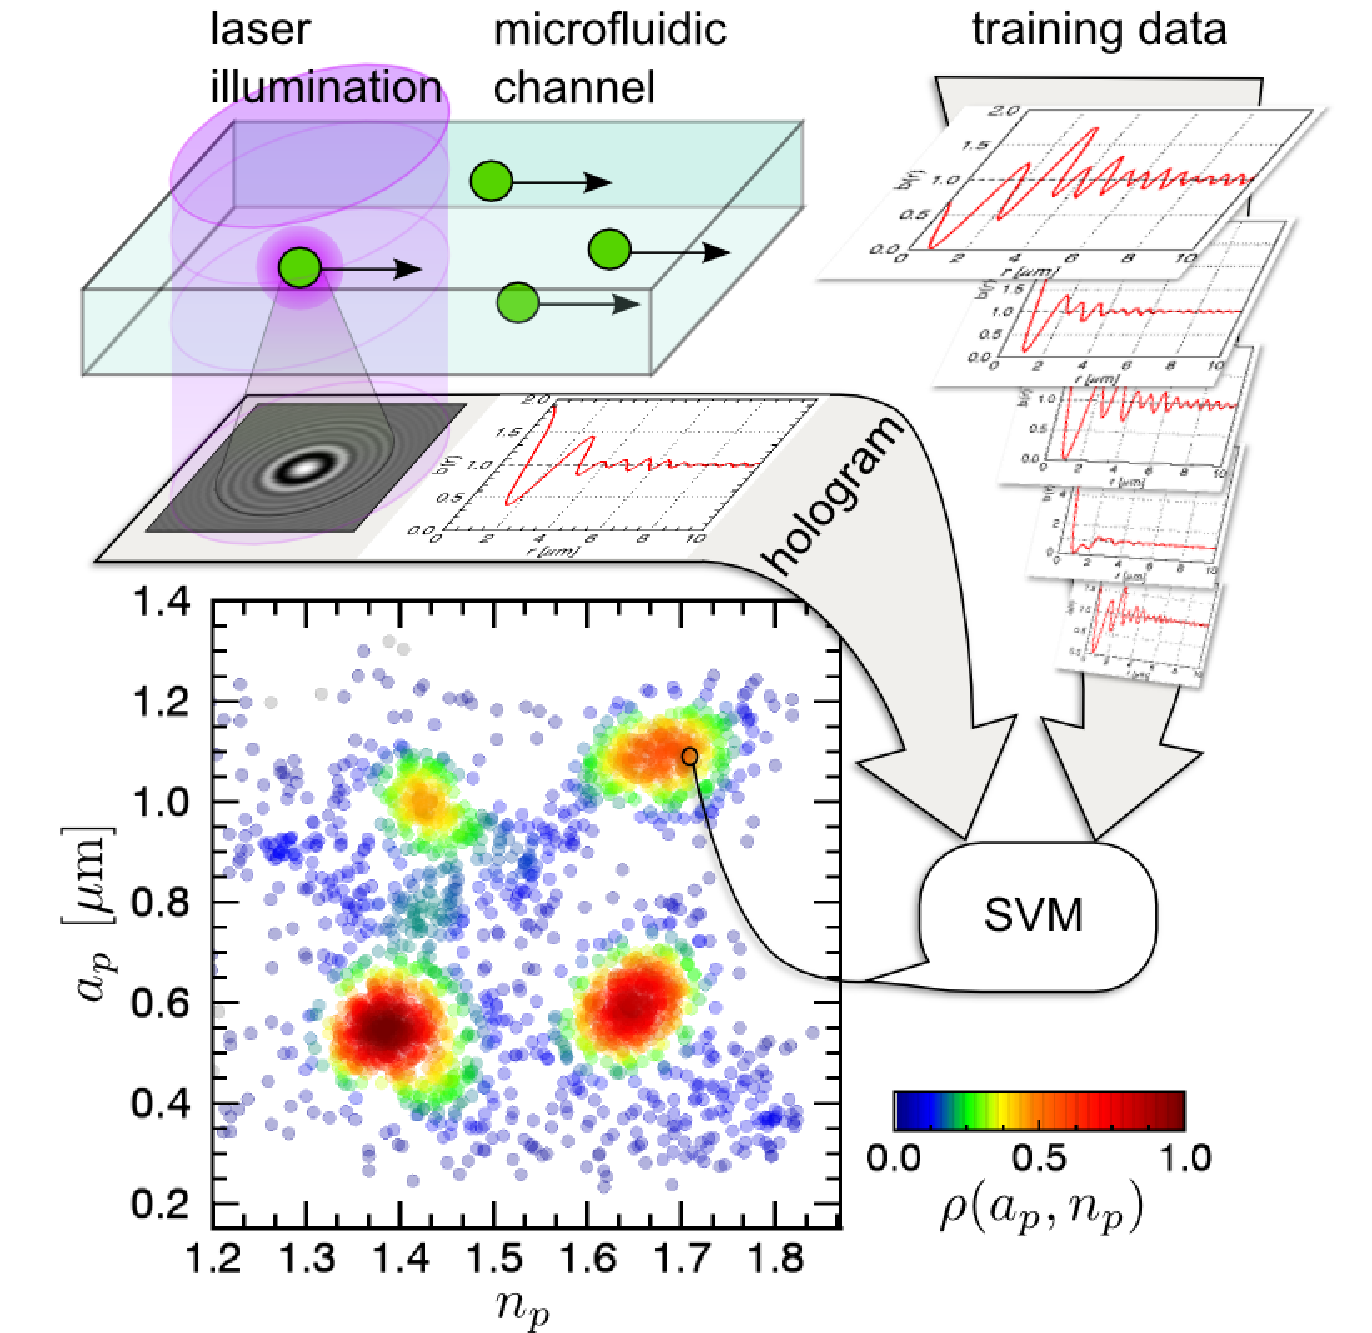
\includegraphics[width=0.7\textwidth]{svr_figure1}
  \caption{Colloidal characterization by holographic microscopy and
    machine learning.  Colloidal spheres flowing down a microfluidic
    sample scatter light from a collimated laser beam to form an
    in-line hologram.  Features in the beam are identified, and their
    radial profiles presented to support vector machines (SVMs)
    that compare them with a library of training data to estimate
    each spheres' radius $a_p$ and refractive index
    $n_p$.  The scatter plot shows results for 2,500 spheres
    drawn at random from a mixture of four different types of
    spheres.  Each point is colored by the local density of
    data points, $\rho(a_p,n_p)$.}
  \label{fig:method}
\end{figure}

\section{Fast Holographic Characterization with Machine Learning}

The in-line holographic microscope used for these studies
\cite{lee07,lee07a,krishnatreya14} 
illuminates the sample with a linearly polarized collimated
laser beam (Coherent Cube, \SI{20}{\mW})
at a vacuum wavelength of
$\lambda = \SI{447}{\nm}$.
The fluence of the \SI{3}{\mm}-diameter beam
is comparable to that of a conventional microscope illuminator.
Optical forces and light-induced heating therefore are negligible.
Light scattered by a sphere
propagates to the focal plane of a custom-built video microscope \cite{krishnatreya14}
where it interferes with the undiffracted portion of the original beam.
The microscope magnifies this interference pattern onto the detector of a greyscale
video camera (NEC TI 324AII), which records its intensity with a system
magnification of \SI{135}{\nm\per pixel}.
Each snapshot in the video stream constitutes a hologram of
the particles in the channel.

The electric field of the incident beam at position $\vec{r}$ in the focal plane
may be modeled as a plane wave with spatial dependence
\begin{equation}
  \label{eq:incidentfield}
  \vec{E}_0(\vec{r}) = u_0(\vec{r}) \, e^{i \varphi_0(\vec{r})} \, e^{i k z} \, \hat{x},
\end{equation}
where $k = 2 \pi n_m / \lambda$ is
the wavenumber in a medium of refractive index $n_m$, and
where $u_0(\vec{r})$ and $\varphi_0(\vec{r})$ account for small variations in the beam's
amplitude and phase profiles, respectively.

A particle located at $\vec{r}_p$ relative to the center of the focal
plane scatters the incident illumination,
$\vec{E}_0(\vec{r}_p)$, to the focal plane as
\begin{equation}
  \label{eq:scatteredfield}
  \vec{E}_s(\vec{r}) 
  = 
  E_0(\vec{r}_p) \, 
  \vec{f}_s\!\left( k (\vec{r} - \vec{r}_p) \vert a_p, n_p \right)),
\end{equation}
where $\vec{f}_s(k\vec{r} \vert a_p, n_p)$ is the Lorenz-Mie scattering function 
\cite{bohren83} that describes how a
sphere of radius $a_p$ and refractive index $n_p$ scatters an $\hat{x}$-polarized plane wave.
The measured
intensity then may be modeled as
\begin{equation}
  \label{eq:intensity}
  I(\vec{r}) 
  = 
  \abs{\vec{E}_0(\vec{r}) + \vec{E}_s(\vec{r})}^2.
\end{equation}
Normalizing the recorded hologram
by $I_0(\vec{r}) = \abs{\vec{E}_0(\vec{r})}^2 = u_0^2(\vec{r})$
suppresses spurious
structure in the illumination
and yields a functional form for the normalized hologram
\cite{lee07a,krishnatreya14},
\begin{equation}
  b(\vec{r}) 
  = \frac{I(\vec{r})}{I_0(\vec{r})}
  \approx
  \abs{
    \hat{x} + 
    e^{-i k z_p} \vec{f}_s(k(\vec{r} - \vec{r}_p)
    \vert a_p, n_p)}^2,
  \label{eq:theory}
\end{equation}
that can be calculated with standard software packages
\footnote{
See, for example, http://physics.nyu.edu/grierlab/software.html for holographic microscopy software written in the IDL programming language that was used in the present study. A comparable implementation in the python programming language is available at http://manoharan.seas.harvard.edu/holopy/.}

Previous implementations of Lorenz-Mie microscopy \cite{lee07a} 
fit Eq.~\eqref{eq:theory} to measured holograms using $a_p$, $n_p$
and $\vec{r}_p$ as adjustable parameters.
These fits are exquisitely sensitive to errors in the particle's
in-plane position, and so must be performed over the entire
two-dimensional intensity distribution \cite{lee07a}.
Here, we instead use Eq.~\eqref{eq:theory} to train
support vector machines, which then are able to estimate 
$a_p$, $n_p$ and $z_p$ from a hologram's one-dimensional
radial profile.
We obtain these profiles from measured holograms by averaging
around centers of rotational symmetry \cite{krishnatreya14a}
with single-pixel resolution, yielding 100-point data vectors.
The microscope's focal plane is adjusted so that the interference
fringes in a typical sphere's hologram extend to roughly this scale.
Averaging over angles to obtain a radial profile reduces the
dimensionality of the analysis problem and accounts in
part for our method's computational efficiency.

Our SVMs are 
implemented with {\tt scikit-learn}, an open-source
machine learning software package \cite{pedregosa11} that
builds upon the {\tt libsvm} library of Support Vector Machine algorithms
\cite{chang01,chang02}.
Each SVM computes one output parameter from an input vector
consisting of a radial profile, $b(r)$, that has been digitized
into 100 single-pixel bins.
Characterizing and tracking a colloidal particle therefore requires
three SVMs, one for each of $a_p$, $n_p$ and $z_p$.
Figure~\ref{fig:method} schematically represents this process
for estimating $a_p$ and $n_p$.

An SVM computes its output by comparing
$b(r)$ with sets of training data, $b_n(r)$,
that are obtained from Eq.~\eqref{eq:theory} over a range
of values of $a_p$, $n_p$ and $z_p$.
Each training set constitutes one support vector in the space 
spanned by these parameters.
To facilitate these comparisons,
we construct SVMs with radial basis functions
\cite{smola04},
\begin{equation}
  \label{eq:5}
  k_n(b)
  =
  \exp\left( -\gamma \int \abs{b_n(r) - b(r)}^2 \, dr \right),
\end{equation}
that quantify the similarity of the experimental input with
the $n$-th support vector.
The sensitivity of this comparison is set by $\gamma$, with
larger values favoring more precise results at the cost of requiring
more support vectors to span the parameter space.
Given a value of $\gamma$,
the training process determines a set of weights $\omega_n$
and an offset $s_0$
such that the weighted sum, 
\begin{equation}
  \label{eq:estimate}
  \tilde{s}(b) = \sum_n \omega_n k_n(b) + s_0,
\end{equation}
constitutes an estimate for the parameter, $s(b)$, that characterizes
the input data vector, $b(r)$.
In general, errors in $\tilde{s}(b)$ depend smoothly
on $\gamma$ \cite{smola04}.

To prevent overfitting, the weights $\omega_n$ are constrained to
have magnitudes less than a maximum value, which conventionally is denoted by
$C$ \cite{smola04}.
Optimizing an SVM with larger values of $C$ improves its ability to recognize its
training data, but renders it less able to interpolate smoothly
between its support vectors when presented with novel or noisy inputs.
Some candidate support vectors may be assigned small weighting
factors in optimizing $\tilde{s}(b)$ over a corpus of training data;
these are automatically eliminated from the SVM \cite{smola04}.
The choice of $\gamma$ and $C$ thus determines which support 
vectors are included in the SVM, and their relative importance for computing the output. 
Because this process is nonlinear, optimal values are obtained by
exhaustive search over the range $0.1 \leq \gamma \leq 10$ and
$0.1 \leq C \leq 1,000$.
Statistically indistinguishable results are obtained in the present application 
for values of $\gamma$ and $C$ that vary from their optimal values by
up to fifty percent. 

We trained SVMs with a 5,000-member training set of radial profiles,
$b_n(r)$, computed with Eq.~\eqref{eq:theory} using the Lorenz-Mie
theory.
Parameters for these computed profiles were evenly distributed over a volume in
the three-dimensional space spanned by
$\SI{13.5}{\um} \leq z_p \leq \SI{75}{\um}$,
$\SI{0.4}{\um} \leq a_p \leq \SI{1.75}{\um}$, and
$1.4 \leq n_p \leq 1.8$ at a resolution of
\SI{1.35}{\um} in $z_p$, 
\SI{0.1}{\um} in $a_p$ and 0.1 in $n_p$.
Training time increases dramatically with 
the number of training sets, and also with larger values of $C$ and $\gamma$.
Once trained, however, an SVM translates input data vectors into 
output parameter estimates extremely rapidly.

The quality of a trained SVM can be assessed by presenting
it with independently computed cross-validation data.
Optimal values for $C$ and $\gamma$ minimize differences
between estimated parameters and the inputs.
Using a 500-member cross-validation set, we obtained
best performance for estimating $z_p$
with $C = 100$ and $\gamma = 1$, best performance
for $n_p$ with $C = 10$ and $\gamma = 0.5$, and
best performance for $a_p$ with $C = 10$ and $\gamma = 0.6$.

Sampling the entire parameter space accessible to
holographic characterization with resolution
comparable to the precision realized with nonlinear fits
\cite{lee07a}
would require more than \num{e10} training sets.
If, however, the system of interest is characterized by a more modest range
of parameters, then results from an initial SVM analysis
can be used to generate a comparatively small set of training data
spanning the relevant range.
This specialized training proceeds rapidly
and yields substantial improvements in precision.

\section{Characterization of Colloidal Mixtures}

The data plotted in Fig.~\ref{fig:method} are
SVM estimates for the radii and refractive indexes of 2,500 
colloidal spheres flowing down a \SI{20}{\um}-deep 
microfluidic channel formed by bonding
the edges of a glass microscope cover slip to the surface of a
glass microscope slide.
The peak flow speed of 
\SI{1}{\mm\per\second} transports  
a sphere across the field of view in no fewer than  
two video frames, ensuring that every particle in the  
flow has a chance to be analyzed.  
Anisotropic blurring due to a sphere's \SI{100}{\nm} 
motion during the camera's \SI{0.1}{\ms} exposure time  
suppresses contrast along the direction of motion, but does not  
appreciably influence the azimuthal average, $b(r)$ \cite{dixon11}.  
Spurious results arising when 
multiple spheres' interference patterns overlap
contribute outliers to the observed
distribution of particle sizes and refractive indexes.
Such artifacts are minimized by diluting the sample to a volume
fraction less than \num{e-3} so that 
no more than three particles are present in any frame.

The sample was prepared by dispersing roughly equal proportions 
of four types of colloidal spheres in water:
\SI{1}{\um}-diameter and \SI{2}{\um}-diameter 
spheres made of polystyrene (Thermoscientific Catalog No.\ 5100A and 
Bangs Laboratories Catalog No.\ SS04N, respectively) and silica (Duke
Standards Catalog Nos.\ 8100 and 4202A, respectively).
Each of these four populations is monodisperse, with a
standard deviation in the radius of less than 5\%.
%The stock particles' refractive indexes also are found to vary
%by about 1\% relative to the mean, presumably because of
%variations in their density.
This four-component mixture was 
flowed through the
observation volume during a \SI{12}{\minute} interval,
and analyzed particle-by-particle.
Each data point in Fig.~\ref{fig:method} corresponds to an individual 
sphere, and is colored by the local density of measurements.

SVM-mediated holographic characterization clearly identifies
the four populations of particles and provides estimates for their relative abundances.
The mode values of the refractive indexes, $n_p \approx \num{1.4}$ 
and \num{1.6} are consistent with values for silica and polystyrene,
respectively.  Values for the radii, $a_p \approx \SI{0.5}{\um}$
and \SI{1}{\um} are consistent with manufacturers'
specifications.
Characterizing multicomponent dispersions
is a unique capability of holographic particle analysis, and
can be performed with SVMs as fast as 
particles' holograms can be acquired.
This performance is all the more noteworthy because the
distribution of particle properties is built up one particle at a time
and so does not rely on \emph{a priori} assumptions.

Neither the instrument nor the analytical technique requires
extensive calibration.
The wavelength of the laser and the effective magnification can be
calibrated once and used for all samples.
The refractive index of the medium is the only free parameter, 
and often can be obtained separately.
These parameters are used to train the SVMs in advance,
after which they can be used to analyze arbitrary samples
dispersed in the medium.

\section{Tracking and Assessment of Precision}

\begin{figure}
  \centering
  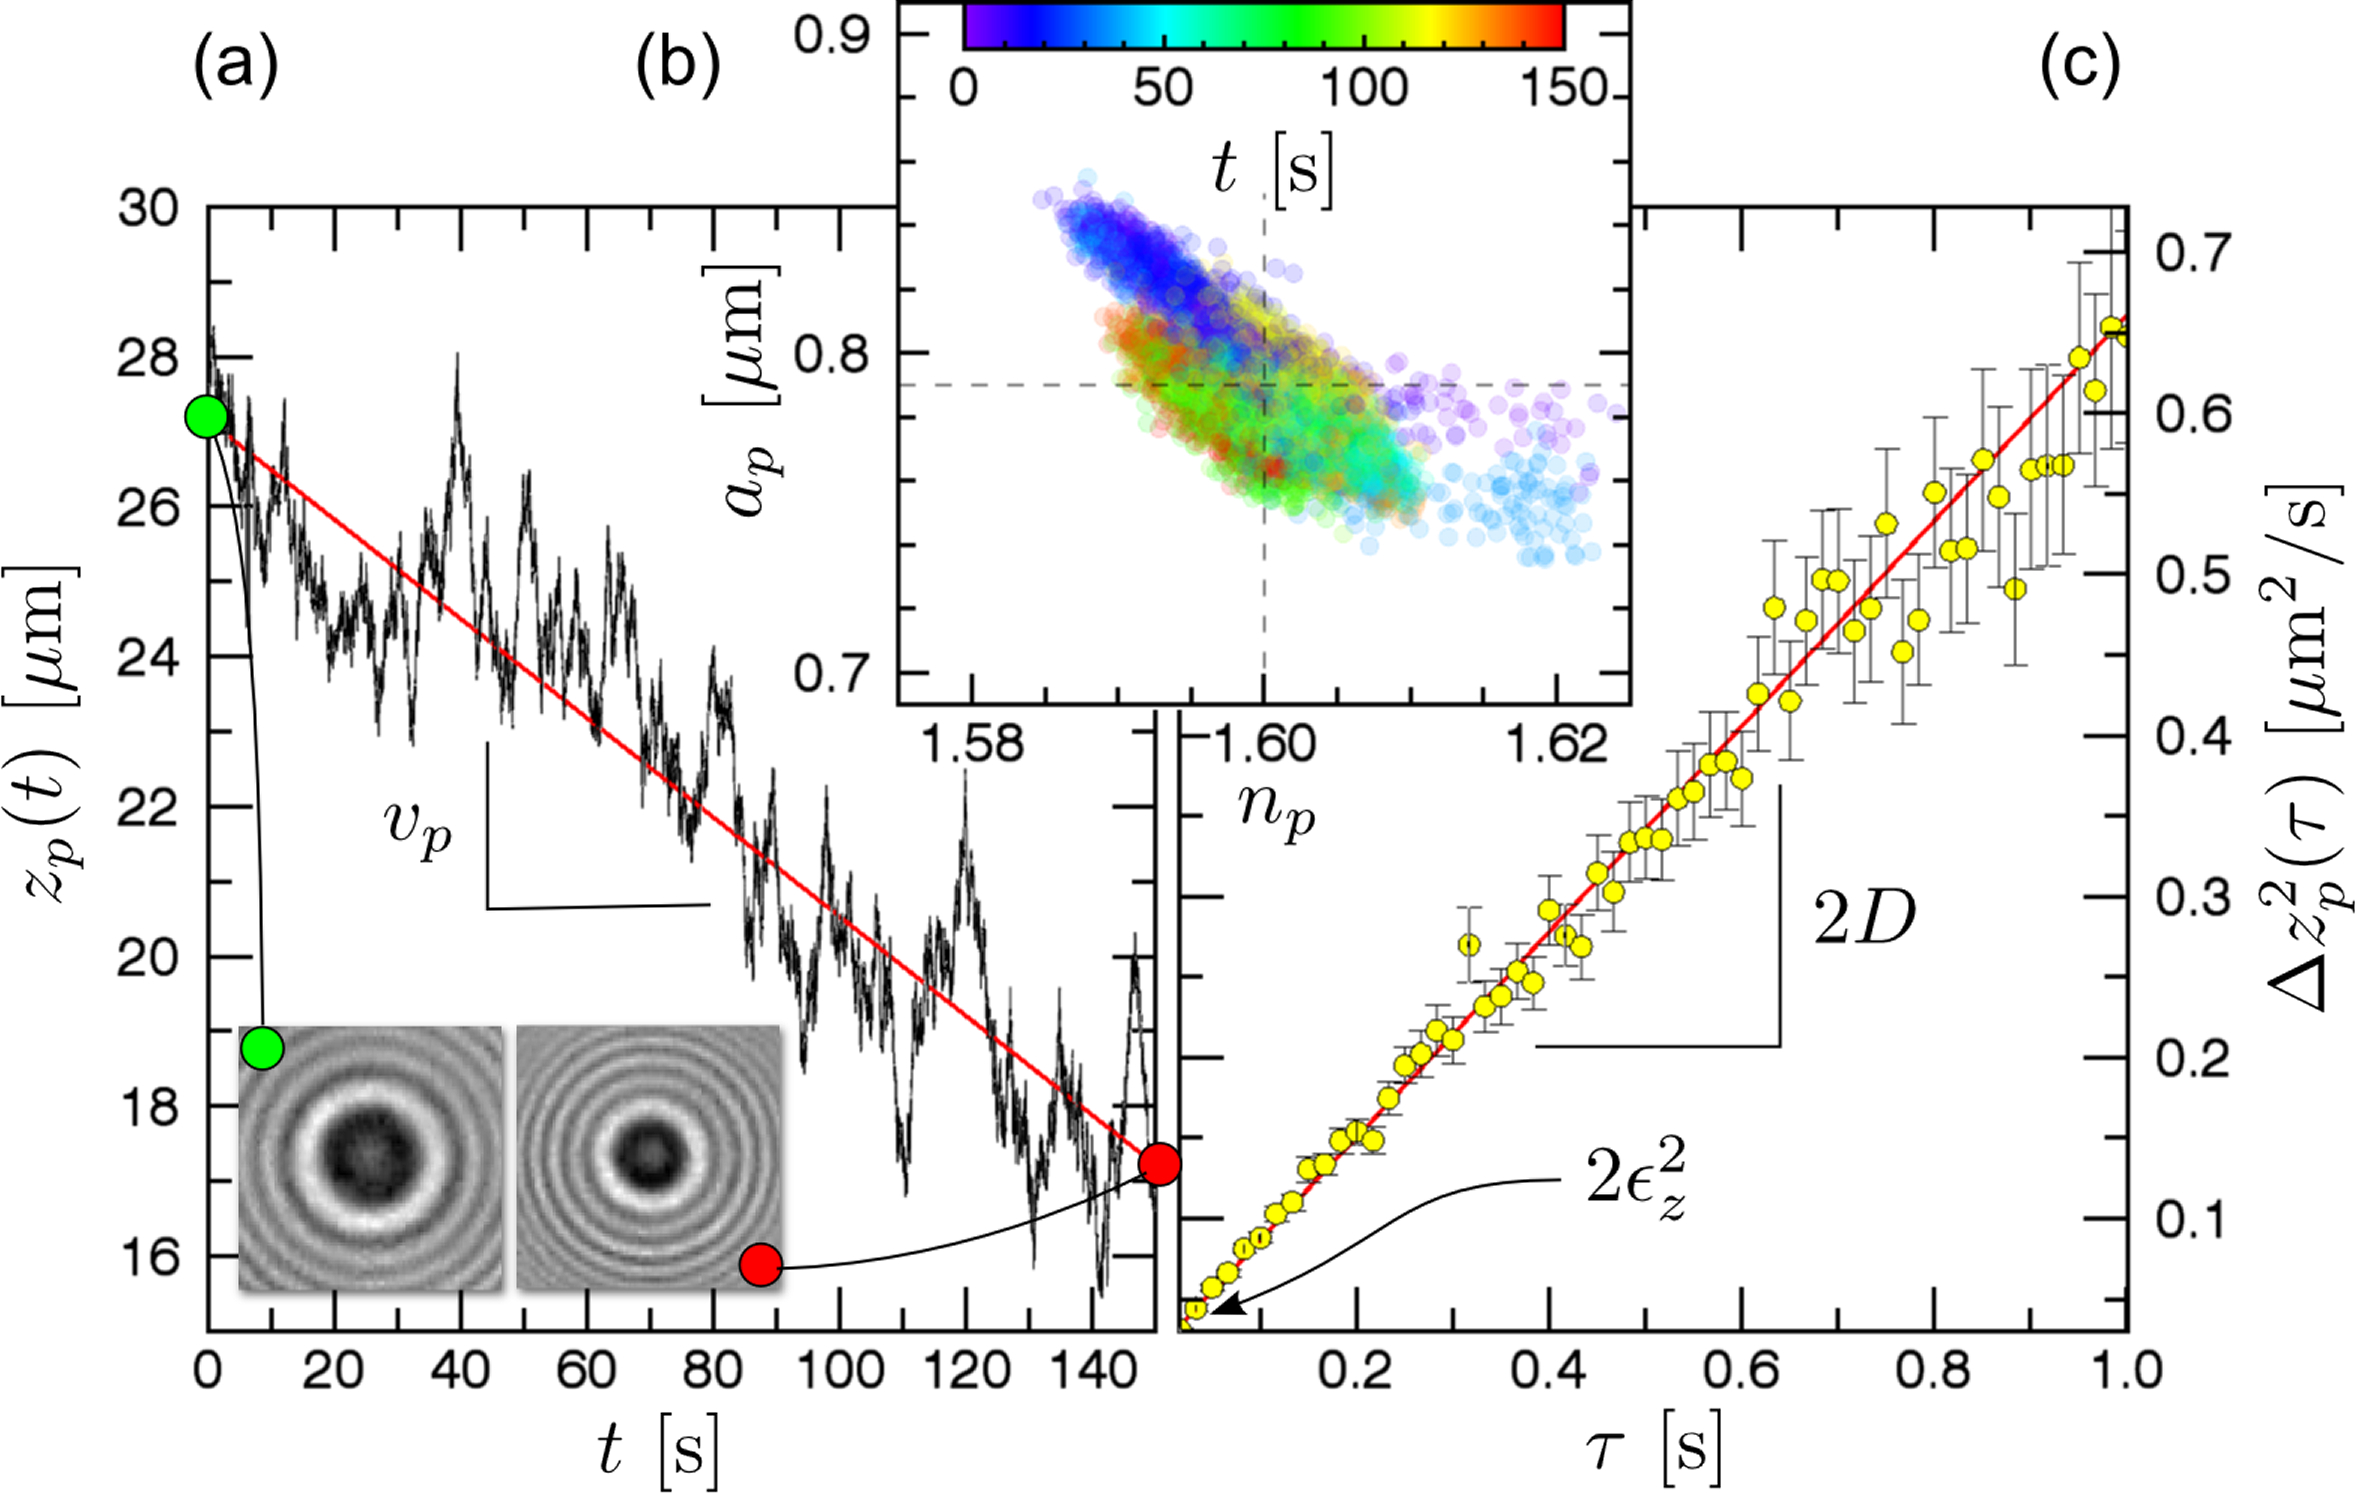
\includegraphics[width=0.9\textwidth]{svr_figure2}
  \caption{Tracking and characterizing a single colloidal sphere.
    (a) The estimated axial position $z_p(t)$ relative to the focal plane
    of the microscope of a single polystyrene sphere sedimenting
    through water as it diffuses.  The line is a least-squares fit.
    Insets show the sphere's hologram at the beginning and end
    of the trajectory.
    (b) The radius $a_p$ and refractive index $n_p$
    estimated from each hologram in the same sequence, colored
    by time.  Each dot corresponds to values obtained from a single
    hologram.
    (c) The mean-squared displacement, $\Delta z_p^2(\tau)$ as a function
    of lag time $\tau$ computed from the data in (a), including
    statistical error bars.  The superimposed line is a fit to
    Eq.~\eqref{eq:einsteinsmoluchowsky}.}
  \label{fig:values}
\end{figure}

Tracking a single colloidal sphere as it sediments and diffuses
provides insights into
the precision and accuracy of SVM-mediated holographic characterization.
The data in Fig.~\ref{fig:values} were obtained with
a \SI{1.59}{\um}-diameter
polystyrene sphere (Duke Scientific, catalog 4016A)
diffusing as it sedimented through
deionized water near the midplane of
a \SI{120}{\um}-deep channel.
Figure~\ref{fig:values}(a) shows the time-resolved
trajectory, $z_p(t)$, obtained from a sequence of 4,500 video frames
recorded at \SI{29.97}{frames\per\second} using iterative
SVM training.

Because polystyrene is roughly 5 percent more dense than water,
the sphere sediments
more that \SI{10}{\um} over the
course of the experiment.
The insets to Fig.~\ref{fig:values}(a) show how markedly
the hologram's appearance changes from the beginning
of the trajectory to the end.
Despite these changes, the SVMs' estimates for the
radius and refractive index plotted in Fig.~\ref{fig:values}(b)
remain clustered around the mean values
$a_p = \SI{0.79(2)}{\um}$
and 
$n_p = \num{1.600(6)}$.

Uncertainties in estimated parameters are computed as
standard deviations of the distribution of results
plotted in Fig.~\ref{fig:values}(b).
These should be interpreted with care because errors in SVM estimates
need not be independent or normally distributed.
Data points in Fig.~\ref{fig:values}(b) cluster around
different values as the particle descends,
which suggests that different support 
vectors dominate the estimates for $a_p$ and $n_p$
when the sphere is at different axial positions.
Systematic errors in the individual parameters therefore may 
vary with changes in any of the parameters' values.
Even so, the averages of the SVM estimates
are consistent with the manufacturer's specifications,
and differ only slightly from those obtained
with a full Lorenz-Mie analysis of the same data set
\cite{krishnatreya14},
which yields $a_p = \SI{0.805(1)}{\um}$ and
$n_p = \num{1.5730(6)}$.
Nonlinear fitting offers ten times better precision and
accuracy \cite{krishnatreya14}.
SVM analysis is a thousand times faster.

The mean sedimentation speed,
$v_p = \SI{66(1)}{\nm\per\second}$,
estimated from the slope of $z_p(t)$ is somewhat smaller than the value measured with
fits to the Lorenz-Mie theory
\cite{krishnatreya14} of $\SI{75(1)}{\nm\per\second}$.
This discrepancy further suggests that the SVM estimate for a
parameter's value may depend on the value itself.
If we nevertheless assume that errors in $z_p$
are normally distributed with a root-mean-square value $\epsilon_z$,
then the diffusing particle's mean-squared
displacement should evolve over time interval $\tau$ as
\begin{equation}
  \Delta z_p^2(\tau)
  \equiv
  \avg{ \left[ z_p(t + \tau) - z_p(t) \right]^2 }_t
  =
  2 D \tau + v_p^2 \tau^2 + 2 \epsilon_z^2,
  \label{eq:einsteinsmoluchowsky}
\end{equation}
where $D = k_B T / (6 \pi \eta a_p)$ is the Stokes-Einstein
value for the particle's diffusion coefficient.
The data in Fig.~\ref{fig:values}(c) yield
$D = \SI{0.319(4)}{\um\squared\per\second}$, which
is slightly larger than the value of
\SI{0.292(4)}{\um\squared\per\second}
obtained with the full Lorenz-Mie analysis \cite{krishnatreya14}.
The best-fit tracking error,
$\epsilon_z = \SI{107(2)}{\nm}$, exceeds the Lorenz-Mie
bound by an order of magnitude
\cite{krishnatreya14}.

\section{Discussion}

The results presented here are typical of the performance of SVMs
for characterizing and tracking colloidal spheres.
of a wide
variety of compositions and sizes over a large axial range.
The speed and precision of SVM characterization
is ideal for monitoring, feedback control and quality assurance
in any industrial process involving colloidal spheres.
In applications where the greatest precision is required, parameters
estimated with SVMs can be used to initialize nonlinear least-squares
fits.
Starting from such reasonable estimates speeds convergence and
reduces the likelihood of failed fits.
Being able to resolve multimodal distributions
by quickly amassing single-particle measurements
avoids ambiguities inherent in population-averaging
methods such as dynamic light scattering.
Extracting the refractive index as well as the size offers
insights into sample composition that otherwise would
not be available.
SVM-accelerated tracking can be used for real-time
three-dimensional particle-tracking velocimetry \cite{cheong09}.
For applications such as microrefractometry \cite{shpaisman12},
the medium's refractive index, $n_m$, can 
be estimated instead of the particle's.

This combination of capabilities enables new applications.
For example, the distribution of properties in colloidal mixtures
could serve as fingerprints for complex fluid systems, with the
sizes, refractive indexes and relative abundances encoding information
that can be accessed with SVM-mediated holographic
characterization.

Such applications can be realized with comparatively
simple instruments \cite{krishnatreya14} conveying image data
to low-power computers.
Although training SVMs can be computationally intensive,
the data comprising a set of trained SVMs occupies less
than \SI{100}{\mega byte}.
Pre-computed SVMs therefore can be archived and rapidly
retrieved when needed.
This approach lends itself to
implementation on embedded computers for integration into
low-cost analytical instruments.

Other machine-learning techniques also might be effective
for analyzing holograms of colloidal particles.  Artificial
neural networks, for instance, can be trained in the same
manner as the present SVM implementation to interpret
radial profiles of experimental holograms.  SVMs have the advantage
that their training process proceeds deterministically, and therefore
tends to be faster.  Once successfully trained, however, artificial
neural networks are generally more computationally efficient.
Regardless of implementation, the present results demonstrate
that machine-learning methods facilitate
fast and precise measurements of colloidal properties.
